\documentclass[a4paper,11pt]{book}
%\documentclass[a4paper,twoside,11pt,titlepage]{book}
\usepackage{listings}
\usepackage[utf8]{inputenc}
\usepackage[spanish]{babel}

% \usepackage[style=list, number=none]{glossary} %
%\usepackage{titlesec}
%\usepackage{pailatino}

%\decimalpoint
\usepackage{dcolumn}
\usepackage{float}
\newcolumntype{.}{D{.}{\esperiod}{-1}}
\makeatletter
%\addto\shorthandsspanish{\let\esperiod\es@period@code}
\makeatother


%\usepackage[chapter]{algorithm}
\RequirePackage{verbatim}
%\RequirePackage[Glenn]{fncychap}
\usepackage{fancyhdr}
\usepackage{graphicx}
\usepackage{afterpage}

\usepackage{longtable}

\usepackage[pdfborder={000}]{hyperref} %referencia

% ********************************************************************
% Re-usable information
% ********************************************************************
\newcommand{\myTitle}{Trabajo Investigación SOA\xspace}
\newcommand{\myDegree}{MÁSTER EN INVESTIGACIÓN EN INGENIERÍA DE SOFTWARE Y
SISTEMAS INFORMÁTICOS\xspace}
\newcommand{\myName}{César Hugo Bárzano Cruz\xspace}
\newcommand{\myProf}{Nombre Apllido1 Apellido2 (tutor1)\xspace}
\newcommand{\myOtherProf}{Nombre Apllido1 Apellido2 (tutor2)\xspace}
%\newcommand{\mySupervisor}{Put name here\xspace}
\newcommand{\myFaculty}{ Universidad Nacional de Educación a Distancia\xspace}
\newcommand{\myFacultyShort}{UNED-Facultad de informática\xspace}
\newcommand{\myDepartment}{\xspace}
\newcommand{\myUni}{\protect{ Universidad Nacional de Educación a Distancia}\xspace}
\newcommand{\myLocation}{Madrid\xspace}
\newcommand{\myTime}{\today\xspace}
\newcommand{\myVersion}{Version 0.1\xspace}


\hypersetup{
pdfauthor = {\myName hugobarzano@gmail.com},
pdftitle = {\myTitle},
pdfsubject = {},
pdfkeywords = {},
pdfcreator = {LaTeX con el paquete TEXmaker},
pdfproducer = {pdflatex}
}

%\hyphenation{}


%\usepackage{doxygen/doxygen}
%\usepackage{pdfpages}
\usepackage{url}
\usepackage{colortbl,longtable}
\usepackage[stable]{footmisc}
%\usepackage{index}

%\makeindex
%\usepackage[style=long, cols=2,border=plain,toc=true,number=none]{glossary}
% \makeglossary

% Definición de comandos que me son tiles:
%\renewcommand{\indexname}{Índice alfabético}
%\renewcommand{\glossaryname}{Glosario}

\pagestyle{fancy}
\fancyhf{}
\fancyhead[LO]{\leftmark}
\fancyhead[RE]{\rightmark}
\fancyhead[RO,LE]{\textbf{\thepage}}
\renewcommand{\chaptermark}[1]{\markboth{\textbf{#1}}{}}
\renewcommand{\sectionmark}[1]{\markright{\textbf{\thesection. #1}}}

\setlength{\headheight}{1.5\headheight}

\newcommand{\HRule}{\rule{\linewidth}{0.5mm}}
%Definimos los tipos teorema, ejemplo y definición podremos usar estos tipos
%simplemente poniendo \begin{teorema} \end{teorema} ...
\newtheorem{teorema}{Teorema}[chapter]
\newtheorem{ejemplo}{Ejemplo}[chapter]
\newtheorem{definicion}{Definición}[chapter]

\definecolor{gray97}{gray}{.97}
\definecolor{gray75}{gray}{.75}
\definecolor{gray45}{gray}{.45}
\definecolor{gray30}{gray}{.94}

\lstset{ frame=Ltb,
     framerule=0.5pt,
     aboveskip=0.5cm,
     framextopmargin=3pt,
     framexbottommargin=3pt,
     framexleftmargin=0.1cm,
     framesep=0pt,
     rulesep=.4pt,
     backgroundcolor=\color{gray97},
     rulesepcolor=\color{black},
     %
     stringstyle=\ttfamily,
     showstringspaces = false,
     basicstyle=\scriptsize\ttfamily,
     commentstyle=\color{gray45},
     keywordstyle=\bfseries,
     %
     numbers=left,
     numbersep=6pt,
     numberstyle=\tiny,
     numberfirstline = false,
     breaklines=true,
   }

% minimizar fragmentado de listados
\lstnewenvironment{listing}[1][]
   {\lstset{#1}\pagebreak[0]}{\pagebreak[0]}

\lstdefinestyle{CodigoC}
   {
	basicstyle=\scriptsize,
	frame=single,
	language=C,
	numbers=left
   }
\lstdefinestyle{CodigoC++}
   {
	basicstyle=\small,
	frame=single,
	backgroundcolor=\color{gray30},
	language=C++,
	numbers=left
   }


\lstdefinestyle{Consola}
   {basicstyle=\scriptsize\bf\ttfamily,
    backgroundcolor=\color{gray30},
    frame=single,
    numbers=none
   }


\newcommand{\bigrule}{\titlerule[0.5mm]}


%Para conseguir que en las páginas en blanco no ponga cabecerass
\makeatletter
\def\clearpage{%
  \ifvmode
    \ifnum \@dbltopnum =\m@ne
      \ifdim \pagetotal <\topskip
        \hbox{}
      \fi
    \fi
  \fi
  \newpage
  \thispagestyle{empty}
  \write\m@ne{}
  \vbox{}
  \penalty -\@Mi
}
\makeatother

\usepackage{pdfpages}
\begin{document}
\begin{titlepage}
 
 
\newlength{\centeroffset}
\setlength{\centeroffset}{-0.5\oddsidemargin}
\addtolength{\centeroffset}{0.5\evensidemargin}
\thispagestyle{empty}

\noindent\hspace*{\centeroffset}\begin{minipage}{\textwidth}

\centering

\includegraphics[width=0.7\textwidth]{imagenes/Logo-uned.jpg}\\[1.1cm]


{\Huge\bfseries Máster Universitario En Investigación En Ingeniería De Software Y Sistemas Informáticos\\
}
\noindent\rule[-1ex]{\textwidth}{3pt}\\[3.5ex]
{\large\bfseries Generación Automática de Código}
\end{minipage}

\vspace{2.5cm}
\noindent\hspace*{\centeroffset}\begin{minipage}{\textwidth}
\centering

\textbf{Autor}\\ {César Hugo Bárzano Cruz}\\[2.5ex]


\includegraphics[width=0.3\textwidth]{imagenes/Logo-master.png}\\[0.1cm]
\textsc{Trabajo 1 De Evaluación Continua}\\
\textsc{---}\\
2017/2018
\end{minipage}
%\addtolength{\textwidth}{\centeroffset}
%\vspace{\stretch{2}}
\end{titlepage}




%\frontmatter
\tableofcontents
\listoffigures
%\listoftables

%
%\mainmatter
%\setlength{\parskip}{5pt}

%\input{capitulos/01_Introduccion}


\chapter{Introducción}

El presente documento representa la memoria formal para el trabajo de investigación de la asignatura Arquitecturas Orientadas a Servicios. Dicho trabajo consta de 2 partes diferencidas. 

En la primera parte, se daran ejemplos de arquitecturas orientadas a servicios en un contexto laboral y empresarial, haciendo distintcion entre soluciones exitosas y soluciones no tan funcionales. En la segunda parte se abordará de una manera más práctica el analisis, diseño e implementación de una arquitectura orientada a servicios con el objetivo de solucionar el problema planteado con este tipo de arquitecturas así como las tecnologías relacionadas con ellas. 

\chapter{Introducción 2}

En la actualidad, las tecnolgías web así como las soluciones basadas en servicios cloud han tomado un gran peso tanto en nuestra vida cotidíana como para el mundo empresarial. El paradigma de servicios cloud denominado "La WEB 2.0" ha revolucionado la manera en la que la información llega al usuario.  El valor aportado al mundo empresarial por el tratamiendo de datos para la toma de decisiones junto con la trasnformación digital ha hecho que innumerables empresas se suban al  carro de las nuevas tecnologías ya que una pequeña inversión en innovación marca una notable mejora en los procesos empresariales.

...etc...CONMPLETAR


\chapter{Soluciones Empresariales SOA}

Cada vez son más las soluciones basadas en arquitecturas orientadas a servicios que el usuario tiene a su disposición y cada vez son más diversas las necesidades tecnológicas que el usuario requiere. Por ello, en los ultimos años, han surgido ciertos proveedores de servicios con soluciones basadas en SOA que se han convertido en el buque insignia de las tecnología cloud. Los proveedores de soluciones para "La WEB 2.0" que se tratarán a continuación son:  


\begin{enumerate}
\item \textbf{Google Cloud Platform}
\item \textbf{Amazon Web Services}
\item \textbf{Microsoft Azure}
\item \textbf{Mlab}
\item \textbf{Yahoo!}
\end{enumerate}

De manera adicional se comentará brevemente Ether Cloud Services, la plataforma de cloud hibrida con base de gobierno presentada por el banco BBVA para este 2018 en el congreso Ether.io de noviembre, plataforma en la que actualmente desempeño el rol de desarrollador de soluciones. 



\subsection{Google Cloud}

Google Cloud Platform, es una plataforma en la nube que ha unificado las aplicaciones para el desarrollo de aplicaciones cloud ofrecidas por Google. Permite crear soluciones  eficientes y escalables. Ejemplos de aplicaciones basadas en SOA pueden ser las propias ofertadas por Google ya que estan basadas en su infraestructura cloud: 

\begin{enumerate}
\item \textbf{Gmail}
\item \textbf{Google Drive}
\item \textbf{Google Sites}
\item \textbf{Google Contacts}
\item \textbf{Google Apps para educación}
\end{enumerate}

Aunque Google pone a disposición de los usuarios bastantes aplicaciones o servicios de caracter gratuito, el principal problema para los desarrolladores de arquitecturas basadas en microservicios es la facturación. Esta puede ser por unidades de cómputo o almacenamiento por lo que un correcto analisis y diseño de la infraestructura virtual que va a soportar la arquitectura basada en servicios que el desarrollador o desarrolladores han de implementar, asi como un análisis del tráfico o concurrencia que dicha SOA ha de soportar puede suponer una correcta decisión o no el usar los servicios cloud ofertados por Google. 

Se considera una SOA exitosa debido al número de usuarios activos que dicha plataforma tiene en todo el mundo, así como la adecuada experiencia de usuario que ofrece. 

\subsection{Amazon Web Services}

AWS es una colección de servicios cloud ofrecidos por Amazon bajo el abanico de su nube pública.  (también llamados servicios web) que en conjunto forman una plataforma de computación en la nube, ofrecida a través de Internet. Algunos ejemplos exitosos de aplicaciones basadas en SOA que a su vez hacen uso de una arquitectura orientada a servicios como ofrece la plataforma de Amazon son:

\begin{enumerate}
\item \textbf{Dropbox}
\item \textbf{Foursquaree}
\item \textbf{HootSuite}
\end{enumerate}

La principal ventaja y a la vez problema de la nube de Amazon es su categorización de servicio por regiones o zonas de disponibilidad que se indican en la tabla de abajo. La división de sus usuarios en las requiones que por localización geográfica mejor servicio ofrezca produce una experiencia de usuario realmente buena, equilibrando el trafico de su infraestructura cloud pero debido a las distintas legislaciones en cuanto a la protección de datos, hay ciertas regiones en las que el almacenamiento masivo de datos de caracter sensible conlleva ciertas responsabilidades. Por ejemplo un desarrollador financiero no siempre podrá alojar sus servicios en l región de disponibilidad que el considere mejor para la latencia del mismo, si no que le vendrá impuesta por contrato o proyecto. 

Se considera un ejemplo de arquitectura basada en servicios muy exitosa debido al gran número de usuario que tiene en todo el mundo. De manera adicional, AWS facilita el aprendizaje de su tecnología a estudiantes proporcionando horas de cómputo y unidades de almacenamiento a los propietarios de cuentas de correo universitario. 

TABLA ZONAS DISPONIBILIDAD

\subsection{Microsoft Azure}

Microsoft Azure es conjunto de servicios cloud de caracter empresarial para solucines comerciales. Azure cuenta con un amplio abanico de servicios, herramientas y frameworks para la creación y administracion de soluciones web a nivel mundial. Se le considera un triunfador en el mundo se los servicios cloud, con su gigantesca arquitectura basada en servicios se presenta como un pionero en el mundo de las soluciones cloud. A pesar de que Azure facilita el aprendizaje de su tecnología a los estudiantes concediendo paquetes de computo se la considera una de las plataformas cloud mas caras en terminos de computo y almacenamiento. 

\subsection{mLab}

mLab se caracteriza por ser un servicio de base de datos cloud que ofrece capacidad de almacenamiento en forma de base de datos relacional, MongoDB. mLab proporviona a sus usuarios un servicio de base de datos no relacional totalmente administrado que se ejecuta sobre proveedores de servicio como los vistos anteriormente (Google, Amazon o Microsoft Azure)

Se considera un ejemplo de SOA exitoso debido a que el servicio ofertado es consumido por miles de desarrolladores cloud en todo el mundo para implementar soluciones SOA ademas de facilitar el aprendizaje de su tecnología de negocio ya que ofrece pequeñas parcelas de almacenamiento cloud de manera gratuita. 

\subsection{Yahoo!}

Yahoo es un portal de internet que ofrece distintos servicios de información como correo electrónico, directorio de servicios web y principalmente motor de busqueda. La arquitectura de este portal esta basada en el paradigma de las arquitecturas basadas en microservicios pero es considera como un fracaso empresarial ya que en En 2009, Yahoo anunció que en el primer trimestre sus utilidades cayeron 78\% con respecto a igual periodo de 2008. La compañía despidió a más de 5\% de su personal, equivalente 700 empleados, que se sumaban a 
los 1500 anunciados el mismo año. La compañía no podía hacer frente a Google, su principal rival por lo que en 2012 despidío a 2000 empleados, el 14\% de su equipo global. 

\subsection{Ether Cloud Services}

ECS se presenta como el futuro competidor de AWS y Google Cloud para desarrolladores de servicios y soluciones financieras sobre escenarios cloud. La plataforma ECS presenta un conjunto de diversas disciplinas de servicios cloud con base de gobierno para el desarrollo y despliegue de aplicaciones basadas en servicios. La plataforma en si es una arquitectura SOA pura en la que un conjunto de piezas o servicios, implementando unas interfaces o End-points comunes son capaces de formar una red cloud a nivel global para ofrecer todo tipo de servicios para desarrolladores de aplicaciones financieras, analisis continuo de flujos de datos, categorización, aprovisionamiento, testing, cómputo y almacenamiento en todo el mundo, permitiendo asi que los procesos de negocio del banco cambien de modo BATCH a REAL TIME.  

\chapter{Aplicación Técnica SOA}

Como segunda parte del trabajo de investigación se va a realizar la especificación, análisis e implementación de un sistema cuya arquitectura esta basada en servicios. 

\section{El Problema}

Como desarrolladores de soluciones, cliente ha solicitado un sistema para el tratamiento y procesamiento de datos. Cliente indica que el producto ha de ser capaz de manejar distintos conjuntos de datos muy variados. De manera adicional, el producto resultante ha de ser capaz de realizar ciertas operaciones sobre los conjuntos de datos. Una de las principales preocupaciones del cliente es su escalabilidad ya que en etapas tempranas del proyecto, el sistema no tendrá mucho tráfico pero en versiones futuras, el número de usuarios a los que tendrá que dar servicio podría expresarse en terminos globales, por lo que el sistema ha de ser rápido, eficiente y facilmente escalable.

\section{Análisis del Problema}

Para abordar el problema planteado por cliente, se ha decidido utilizar una arquitectura basada en microservicios. Para ello, se pretende definir un bloque principal para la gestión de los conjuntos de datos o datasets. Cliente será capaz de interaccionar con el bloque de gestión mediante una API-RESTFUL basada en protocolo http, lo que le permitirá consumir el servicio de datos y usar el sistema como back-end para implementar aplicaciones que consuman dicho servicio de tratamiento de datos de una manera sencilla y homogenea. De manera adicional y usando dicha interfaz REST, el cliente será capaz de realizar operaciones sobre los conjuntos de datos que  el sistema es capaz de gestionar. Con el objetivo de optimizar el rendimiento y la eficiencia se ha decidido delegar el procesamiento de datos a otro servicio totalmente independiente al bloque principal de gestión, por lo que tanto el bloque de gestión como los servicios esclavos encargados del tratamiento de datos, deberan implementar una API-REST privada. De esta forma, la experiencia que percibe el usuario será trasnparente al procesamiento que el sistema realice en su interior, ya que cliente solo conocerá la API publica del bloque de gestión. 

Este paradigma permitirá al sistema escalar fácilmente e incluir nuevas operaciones o tratamientos para los datos que el bloque de gestión disponibiliza mediante la API pública a cliente. El siguiente diagrama muestra la arquitectura basada en servicios rest que se quiere desarrollar para solucionar el problema propuesto. 


\begin{figure}[H]  
\centering 
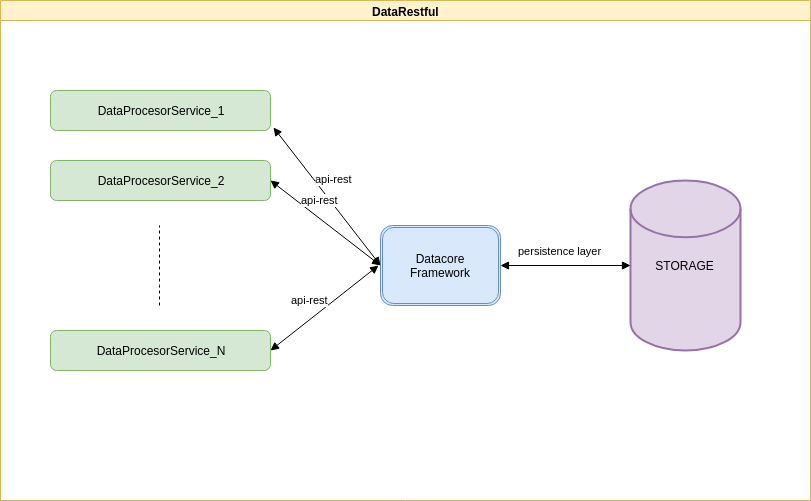
\includegraphics[scale=0.35]{imagenes/arquitectura_datarest.png}
\caption{ Arquitectura SOA }  
\end{figure} 

Podemos distinguir 3 elementos o conceptos principales dentro del sistema propuesto, bautizado como Datarestful:

\begin{enumerate}
\item \textbf{Procesadores}
\item \textbf{Datacore}
\item \textbf{Almacenamiento}
\end{enumerate}


Para el usuario y su experiencia con el sistema, esto es transparente pues el realizará peticiones a Datarestful nivel sistema mediante la Api pública expuesta por el Datacore o framework a nivel sub-sistema y delegadas al resto del subsistemas dependiendo de si se requiere cómputo, almacenamiento o ambos mediante la Api privada no accesible para ususarios, si no solo para los servicios que formen parte de la aquitectura SOA que forma Datarestful. 

\subsection{Procesadores}

Encargados del procesamiento y tratamiendo de datos, son los encargados del procesamiento y tratamiento de datos, ofrecen servicio al core del sistema mediante Api-rest privada. Su objetivo es la computación por lo que carecen de capa de persistencia, reciben conjuntos de datos y devuelven el resultado de aplicar cierta operación sobre ese conjunto de datos. 

\subsection{Datacore}

Framework encargado de gestionar los conjuntos de datos, su tarea es la de proporcionar al usuario una interfaz rest para manejar los datos y solicitar operaciones sobre los mismos. Carece de capacidad computacional pues todas las operaciones son delegadas a los servicios de procesamiento registrados en él. Datacore es el encargado de interactuar con la capa de persistencia implementando las operaciones CRUD necesarias para interactuar con la base de datos.  

\subsection{Storage}

Capa de persistencia encargada del almacenamiento de datos.  

\section{Especificación de la Solución}

Tras analizar el problema a resolver, en esta seción se realizará la espeficación necesaria para su solución. Para ello, se van a definir los siguientes subsecciones: 

\subsection{Requisitos de Información del Sistema}

Los requisitos de información se caracterizan por reunir la información relevante para el cliente, es decir, que debe gestionar y almacenar el sistema software.\\

\textbf{RI-1. Dataset:} Representación de cada uno de los conjuntos de datos en el sistema. 
Contenido: ID unico del conjunto de datos, título representativo del dataset, fecha de creación y el conjunto de datos en si. \\


\textbf{RI-2. Operación:} Representación de cada una de las operaciones comptacionales que el sistema pone a disposición del ususario. Contenido: ID único de la operacion, operador o palabra reservada para realizar la operación, número de datasets que estan involucrados en la operación. \\

\subsection{Requisitos Funcionales del Sistema}

Como se define en la ingeniería de requisitos, los requisitos funcionales establecen los comportamientos del sistema.\\ 

\textbf{RF-1. Gestión de datasets:} El sistema será capaz gestionar el ciclo de vida de los datasets existentes en el sistema.\\
   

	RF-1.1. El sistema permitirá añadir datasets.

	RF-1.2. El sistema permitirá buscar datasets.

	RF-1.3. El sistema permitirá modificar datasets.

	RF-1.4. El sistema permitirá eliminar datasets.


\textbf{RF-2. Tratamiento de Datos:} El sistema deberá disponibilizar al usuario una serie de operaciones sobre los conjuntos de datos. \\   


	RF-2.1. El sistema permitirá realizar una operacion sobre uno o mas conjuntos de datos. 

	RF-2.2. El sistema permitirá consultar las operaciones disponibles. 

	RF-2.3. El sistema permitirá crear nuevos conjuntos de datos mediante el resultado de una o más operaciones. 

	RF-2.4. El sistema permitirá programar operaciones para ser realizadas en determinados momentos del día. 
	
\subsection{Requisitos No Funcionales del Sistema}

Los requisitos no funcionales, se refieren a todos los requisitos que no describen información a guardar, ni funciones a realizar por el sistema, sino características de funcionamiento.\\


\textbf{RNF-1} Necesitaremos que toda la información que se almacena sobre el sistema se mantenga segura, realizando copias de seguridad periódicas. \\

\textbf{RNF-2} Necesitaremos que los conjuntos de datos esten disponibles de manera rápida. \\

\textbf{RNF-3} Necesitaremos disponer de una buena conexión a internet ya que el sistema da servicio desde la nube. \\ 


\section{Implementación y Tecnológia}

Una vez realizado el análisis del problema y especificada la posible solución es el momento de tomar las decisiones adecuadas para la correcta implementación de Datarestful. De manera general, los servicios que forman el sistema han de implementar ciertos End-points o interfaces de comunicación que les permita interactuar entre ellos y con el ususario, para ello, se hará uso de HTTP (Hypertext Transfer Protocol) es un protocolo de comunicación que permite las transferencias de información en la web. 

Como se vió en el apartado "Análisis del Problema" hay 3 bloques principales que trataremos a continuación:  

\subsection{Procesadores}

Para la implementación de un procesador basíco al que el sistema pueda solicitar operaciones sobre los datasets, se ha decidido utilizar python, mediante el micro-framework Flask para el desarrollo de aplicaciónes web. Se ha decidido utilizar python como tecnoloǵia base debido a la gran variadad de librerias y algoritmos para el tratamiento de datos que existen para este lenguaje, muchas de ellas son adaptaciones de librerias pertenecientes al popular lenguaje para mineria de datos denominado R. 

La ventaja de la aquitectura basada en servicios que se va a implementar reside en que la tecnología utilizada es independiente al problema, es decir, el sistema puede delegar las operaciones computacionales a distintos servicios de procesado y estos pueden estar implementados con diversas tecnológias como python, javascript, scala...lo unico que han de hacer es implementar los End-points o interfaces rest que se definan en el API privada para que el sistema pueda delegar tareas computacionales a dichos servicios.

\subsection{Datacore}

Como se especificó anteriormente, Datacore es la pieza encargada de orquestar las peticiones de los usuarios con los servicios de cómputo y almacenamiento por eso se ha decidido impementar utilizando el lenguaje de programación GO. Esta tecnología esta orientada al desarrollo de servicios rest de altas prestaciones, optimizando el trafico y las peticiones concurrentes. Al tratarse de un lenguaje compilado, los ejecutables generados son multiplataforma lo que facilita su despliegue sobre diversas infraestructuras. 

\subsection{Store}

Como capa de persistencia se ha decidido utilizar un modelo NO relaccional, lo que permite almacenar datasets como documentos, esto significa que el enrriquecimiento de las estructuras de datos almacenadas puede realizarse de manera simple. Para ello, se ha decidido utilizar el motor NoSql proporcionado por MongoDB. Este software permite optimizar las busquedas de datasets mediante la indexación de sus colecciones de documentos lo que supone una ganacia en eficiencia con respecto a bases de datos relaccionales orientadas a transaciones de objetos como Postgresql o Mysql.        


\begin{lstlisting}[language=python,caption={make testCase1 }]

#!/usr/bin/env bash
export GENERATOR_CONFIG=./input/GAC_GENERATOR_CONFIG_1.json
make build
./generadorP3
python ./output/Consumer_class_generated.py

\end{lstlisting}



 

\begin{thebibliography}{aaaa}

%intro

\bibitem[1]{xml} \textsc{XML},
\textit{XML Format}
\url{https://www.w3.org/XML/} 


\bibitem[2]{json} \textsc{JSON},
\textit{JSON Format}
\url{https://www.json.org/} 

%Desarrollo

\bibitem[3]{py} \textsc{python},
\textit{Python 2.7.6 language}
\url{https://www.python.org/download/releases/2.7.6/} 


\bibitem[4]{json_lib} \textsc{import json},
\textit{JSON encoder and decoder}
\url{https://docs.python.org/2/library/json.html} 

\bibitem[5]{xmltodic_lib} \textsc{import xmltodic},
\textit{Makes working with XML feel like you are working with JSON}
\url{https://pypi.python.org/pypi/xmltodict} 

\bibitem[6]{sys_lib} \textsc{import sys},
\textit{System-specific parameters and functions}
\url{https://docs.python.org/2/library/sys.html} 

\bibitem[7]{os_lib} \textsc{import os},
\textit{Miscellaneous operating system interfaces}
\url{https://docs.python.org/2/library/os.html} 

\bibitem[8]{getopt_lib} \textsc{import getopt},
\textit{C-style parser for command line options}
\url{https://docs.python.org/2/library/getopt.html}


\end{thebibliography}
 

\chapter{Anexo}
\section{generator.py}



%
%
%%\nocite{*}
%\bibliography{bibliografia/bibliografia}\addcontentsline{toc}{chapter}{Bibliografía}
%\bibliographystyle{miunsrturl}
%
%\appendix

%\input{apendices/manual_usuario/manual_usuario}
%%\input{apendices/paper/paper}
%\input{glosario/entradas_glosario}
% \addcontentsline{toc}{chapter}{Glosario}
% \printglossary

\thispagestyle{empty}

\end{document}
